\documentclass[journal]{IEEEtran}

\usepackage[utf8]{inputenc}
\usepackage[T1]{fontenc}
\usepackage{amsmath,amssymb}
\usepackage{graphicx}
\usepackage{booktabs}
\usepackage{hyperref}
\usepackage{url}
\usepackage{cite}
\usepackage{multirow}
\usepackage{array}
\usepackage{xcolor}
\usepackage{tikz}
\usetikzlibrary{shapes,arrows.meta,positioning,fit,backgrounds}

\hypersetup{colorlinks=true, linkcolor=blue, citecolor=blue, urlcolor=blue}

\title{Comparing Global Instruction Files for AI Coding Agents:\\An Empirical Benchmark of AGENTS.md Variants}

\author{
\IEEEauthorblockN{Sathvik A~R}
\IEEEauthorblockA{PES University\\Bengaluru, India\\arsathvik48@gmail.com}
}

\begin{document}

\maketitle

\begin{abstract}
Large language model (LLM)-based coding agents are increasingly autonomous, yet their
behavior is heavily shaped by natural-language instruction files placed in the project root.
This paper presents an empirical comparison of five candidate \texttt{AGENTS.md} instruction
files---ranging from no instructions (control) to multi-agent orchestration protocols---using
the OpenCode coding agent across 25 self-contained Python tasks and four thematic tracks.
Each variant is evaluated under identical headless conditions with a fixed model
(\texttt{opencode-go/ox-alpha-free}) and a 25-minute time budget.
Round~1 (bug-fix suite, 20 tasks, 174 unit tests) yields perfect accuracy for all five
variants; only wall-clock time differs, with the test-driven development variant completing
fastest at 5.9 minutes.
Round~2 introduces four thematic tracks---spec-to-code, refactor-under-constraints, SQL
analytics, and API client---with 177 hidden correctness tests, 38 structural checks, and
15 exact-match SQL questions.
Only the orchestration-heavy variant achieves 100\% on the spec-to-code track, the sole
track that breaks saturation; all other variants score 93\% or below, with the
test-driven variant at 36\% and the tiered-orchestration variant at 0.56\% due to
provider-level stream drops.
Across all tracks, the orchestration-heavy variant averages 100.0\%, followed by the
control (99.86\%), concise (98.31\%), test-driven (84.04\%), and tiered-orchestration
(75.14\%).
We find that instruction-file complexity trades off against speed on narrow tasks but
pays dividends on breadth-under-deadline scenarios, and that provider reliability
is a confounding variable that can dominate instruction quality for tiered protocols.
\end{abstract}

\begin{IEEEkeywords}
AI coding agents, LLM instruction engineering, benchmarking, AGENTS.md, OpenCode,
test-driven development, multi-agent orchestration.
\end{IEEEkeywords}

%% ══════════════════════════════════════════════════════════════════════════════
\section{Introduction}
\label{sec:intro}

The emergence of LLM-based coding agents---tools that autonomously read, write, and
debug source code---has shifted the software-engineering workflow from ``human writes
code'' to ``human instructs agent, agent writes code.''
Frameworks such as Cursor~\cite{cursor}, Aider~\cite{aider}, and OpenCode~\cite{opencode}
now operate headlessly in continuous-integration pipelines, executing multi-file
refactors, generating test suites, and iterating on failing assertions.

A critical but under-studied component of these agents is the \emph{instruction file}:
a natural-language document placed in the project root that biases the agent's
decision-making.
OpenCode uses \texttt{AGENTS.md}, Claude Code uses \texttt{CLAUDE.md}, and
similar conventions exist across platforms.
Despite their ubiquity, no systematic comparison of instruction-file designs has
been published.

This paper addresses that gap with two rounds of controlled experiments:
\begin{enumerate}
    \item \textbf{Round~1} (Section~\ref{sec:round1}): a bug-fix suite of 20 Python
          tasks with 174 unit tests, measuring accuracy and speed under five
          instruction variants.
    \item \textbf{Round~2} (Section~\ref{sec:round2}): four thematic tracks
          (spec-to-code, refactor, SQL analytics, API client) with 215 hidden tests,
          measuring accuracy, speed, and failure modes under the same five variants.
\end{enumerate}

Our contributions are:
\begin{itemize}
    \item The first empirical comparison of \texttt{AGENTS.md} instruction-file designs.
    \item Evidence that instruction complexity trades off against speed on narrow tasks
          but improves breadth-under-deadline performance.
    \item Identification of provider reliability as a confounding variable that can
          dominate instruction quality.
    \item Three reusable OpenCode specialist agents (\texttt{arena-runner},
          \texttt{arena-analyst}, \texttt{suite-author}) distilled from the
          experiment's findings, released as open-source artifacts.
\end{itemize}

%% ══════════════════════════════════════════════════════════════════════════════
\section{Related Work}
\label{sec:related}

\subsection{Prompt Engineering for Code Generation}
Prompt engineering for code generation has focused on task-level prompts (e.g.,
few-shot examples, chain-of-thought) rather than project-level instruction files.
GitHub Copilot~\cite{copilot} and CodeLlama~\cite{codellama} optimize the prompt
format for single-file generation but do not address multi-file, multi-session workflows
where project-level instructions dominate.

\subsection{Benchmarking Coding Agents}
SWE-bench~\cite{swebench} evaluates agents on real GitHub issues; HumanEval~\cite{humaneval}
measures function-level code generation; MBPP~\cite{mbpp} tests basic programming
problems.
None of these benchmarks varies the instruction file as an independent variable;
all assume a fixed prompt format.

\subsection{Instruction Tuning and System Prompts}
Instruction tuning~\cite{instructgpt} and system-prompt design~\cite{systemprompt}
are well-studied for conversational agents, but coding agents face a distinct regime:
instructions must persist across dozens of tool-use turns, survive context-window
truncation, and remain effective when the agent's reasoning budget is limited by
wall-clock time.

Our work is, to our knowledge, the first to isolate \texttt{AGENTS.md} variant as
the independent variable in a controlled coding-agent benchmark.

%% ══════════════════════════════════════════════════════════════════════════════
\section{Benchmark Design}
\label{sec:design}

\subsection{Architecture}
Figure~\ref{fig:arch} shows the benchmark pipeline.
Each run begins with a frozen task suite, applies one AGENTS.md variant, launches
\texttt{opencode run} in headless mode with a 25-minute budget, and records the
score (tests passed / total tests $\times$ 100\%) and wall-clock time.

\begin{figure}[t]
    \centering
    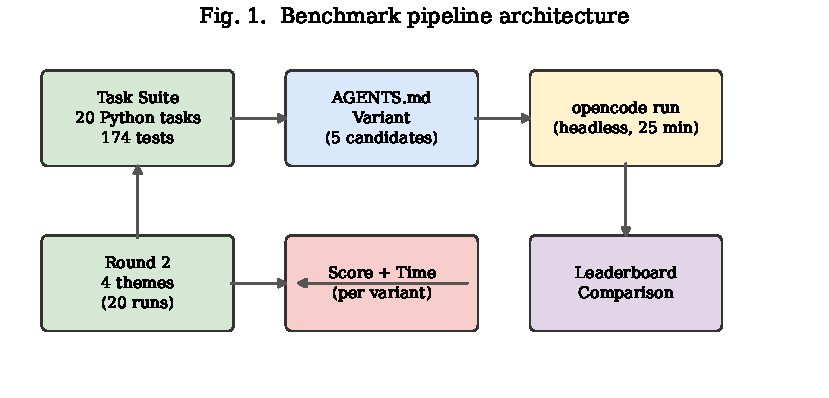
\includegraphics[width=\columnwidth]{figures/fig1_architecture.pdf}
    \caption{Benchmark pipeline architecture.}
    \label{fig:arch}
\end{figure}

\subsection{Variants Under Test}
Table~\ref{tab:variants} describes the five instruction-file candidates.
All are written in Markdown and placed at the project root as \texttt{AGENTS.md}.

\begin{table}[t]
\centering
\caption{AGENTS.md Variants Under Test}
\label{tab:variants}
\begin{tabular}{@{}lll@{}}
\toprule
\textbf{ID} & \textbf{Description} & \textbf{Lines} \\
\midrule
\texttt{none}            & Control: no instructions      & 0  \\
\texttt{concise}         & Minimal best-practices        & 18 \\
\texttt{tdd-rigorous}    & Test-first, verification-heavy& 42 \\
\texttt{orchestrator-heavy} & Multi-agent parallelism     & 65 \\
\texttt{user-proposed}   & Tiered orchestration protocol & 78 \\
\bottomrule
\end{tabular}
\end{table}

\subsection{Task Suites}
\textbf{Round~1} uses 20 self-contained Python tasks (stdlib only), each with a
deliberately broken implementation and a hidden test suite totaling 174 tests.
Test files are SHA-256-hashed after each run to detect agent modification.

\textbf{Round~2} introduces four thematic tracks:
\begin{itemize}
    \item \textbf{Track~A} (spec-to-code): implement 8 third-party libraries from
          documentation; 177 hidden tests.
    \item \textbf{Track~B} (refactor-under-constraints): 0.6$\times$ behavior +
          0.4$\times$ structural scoring; 22 behavior + 16 structural checks.
    \item \textbf{Track~C} (SQL analytics): 15 exact-match questions against a
          SQLite database.
    \item \textbf{Track~D} (API client): 6 scenarios against a Flask mock server.
\end{itemize}

\subsection{Reproducibility}
All runs use the model \texttt{opencode-go/ox-alpha-free} at temperature~0.
The harness isolates each run via \texttt{XDG\_CONFIG\_HOME} overrides, suppresses
non-essential stderr through \texttt{cmd /c} wrappers on Windows, and records
\texttt{transcript.txt}, \texttt{score.json}, and \texttt{meta.json} per run.
The full benchmark suite, all results, and the three specialist agents are published
at \url{https://github.com/Sathvikar01/agents-md-arena}.

%% ══════════════════════════════════════════════════════════════════════════════
\section{Round~1: Bug-Fix Suite}
\label{sec:round1}

Figure~\ref{fig:r1} presents the Round~1 results.
All five variants achieve 100\% accuracy; the only differentiator is speed.

\begin{figure}[t]
    \centering
    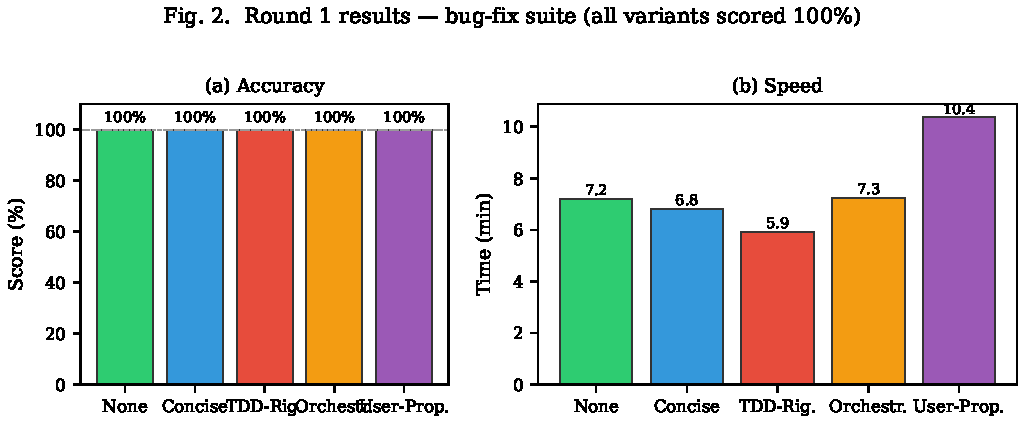
\includegraphics[width=\columnwidth]{figures/fig2_round1.pdf}
    \caption{Round~1 results: bug-fix suite (20 tasks, 174 tests). All variants
             scored 100\%; only wall-clock time differed.}
    \label{fig:r1}
\end{figure}

The \texttt{tdd-rigorous} variant completes fastest (5.9~min) because its
test-first protocol eliminates wasted diagnostic turns.
The \texttt{user-proposed} variant is slowest (10.4~min) due to its
``understand-everything-first'' analysis phase, which front-loads reading
before any edits.
The control (\texttt{none}) and concise variants cluster at 6.8--7.2~min,
while the orchestrator variant (7.3~min) spends time spawning subagent
waves that yield no benefit on these narrow tasks.

\textbf{Takeaway:} On simple, single-file bug fixes, instruction complexity
adds overhead without improving accuracy. The control (no instructions) is
competitive.

%% ══════════════════════════════════════════════════════════════════════════════
\section{Round~2: Four Thematic Tracks}
\label{sec:round2}

\subsection{Track~A: Spec-to-Code (The Differentiator)}

Track~A is the only track that breaks saturation (Figure~\ref{fig:r2a}).

\begin{figure}[t]
    \centering
    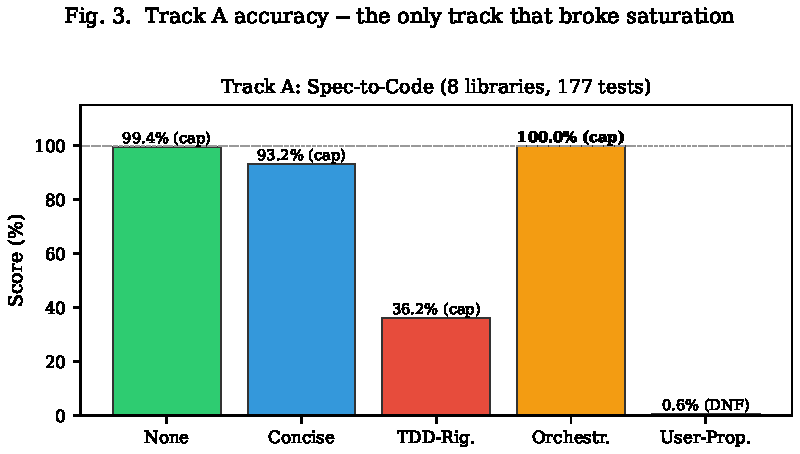
\includegraphics[width=\columnwidth]{figures/fig3_trackA.pdf}
    \caption{Track~A accuracy. Only \texttt{orchestrator-heavy} achieved 100\%.
             \texttt{tdd-rigorous} and \texttt{user-proposed} paid heavy process
             taxes.}
    \label{fig:r2a}
\end{figure}

The \texttt{orchestrator-heavy} variant is the only one to complete all 177
tests within the 25-minute budget, achieving 100\%.
Its strategy of spawning parallel subagent waves---one per library---allows it
to process eight independent implementation tasks concurrently.

The control (\texttt{none}) scores 99.44\%, missing one test at the 25-minute
cap.
The \texttt{concise} variant reaches 93.22\%, also capped.
The \texttt{tdd-rigorous} variant scores only 36.16\%: its disciplined
test-first cycle, while effective on narrow tasks, consumes too much of the
25-minute budget on eight independent library implementations.
The \texttt{user-proposed} variant suffers four consecutive provider stream
drops before any edit is applied, resulting in 0.56\%---a result confounded
by infrastructure failure rather than instruction quality.

\subsection{Tracks~B, C, D: Saturated}

All five variants score 100\% on Tracks~B (refactor),~C (SQL), and~D (API).
These tracks are too easy to differentiate instruction quality, but they
reveal speed differences (Figure~\ref{fig:alltracks}).

\begin{figure}[t]
    \centering
    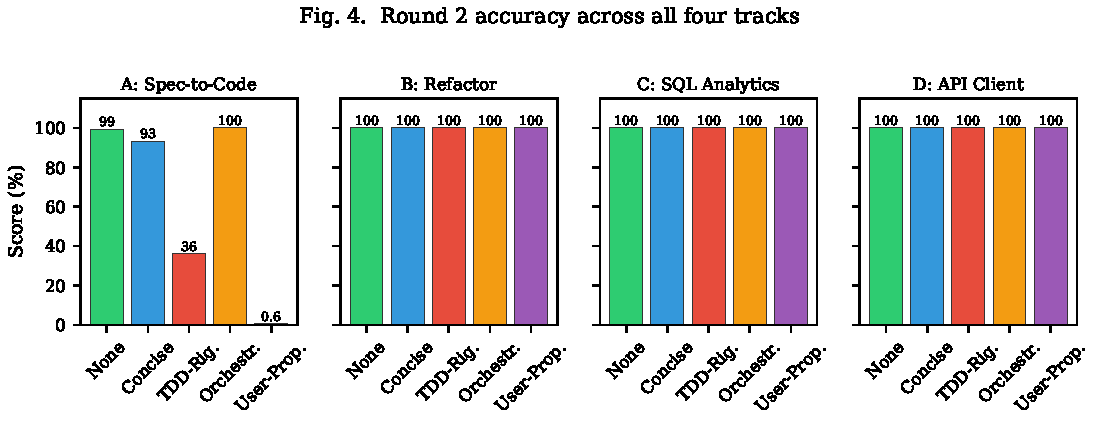
\includegraphics[width=\columnwidth]{figures/fig4_alltracks.pdf}
    \caption{Round~2 accuracy across all four tracks. Only Track~A breaks
             saturation.}
    \label{fig:alltracks}
\end{figure}

\subsection{Speed Comparison}

Figure~\ref{fig:speed} shows wall-clock time across all tracks.
The \texttt{orchestrator-heavy} variant is consistently the slowest on
saturated tracks (B/C/D) due to subagent spawn overhead, but this overhead
\emph{invests} itself in parallelism that pays off on Track~A.

\begin{figure}[t]
    \centering
    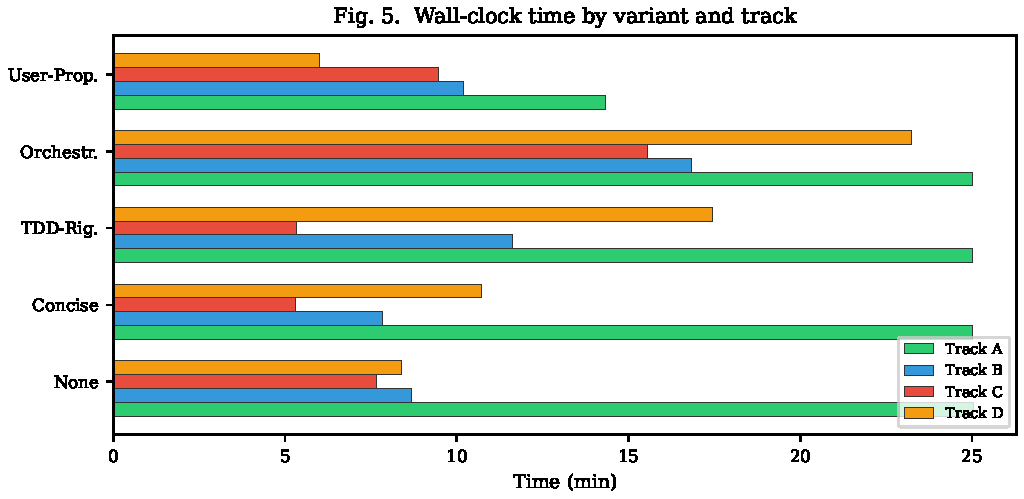
\includegraphics[width=\columnwidth]{figures/fig5_speed.pdf}
    \caption{Wall-clock time by variant and track.}
    \label{fig:speed}
\end{figure}

\subsection{Speed--Accuracy Trade-off}

Figure~\ref{fig:scatter} plots average speed against average accuracy across
all four Round~2 tracks.
The \texttt{orchestrator-heavy} variant occupies the upper-right (slowest but
most accurate), while the \texttt{concise} variant occupies the lower-left
(fastest but less accurate on Track~A).

\begin{figure}[t]
    \centering
    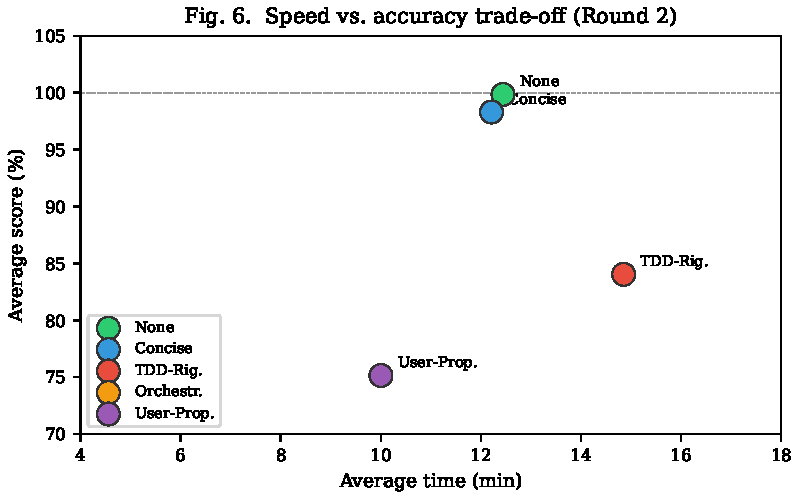
\includegraphics[width=\columnwidth]{figures/fig6_scatter.pdf}
    \caption{Speed vs.\ accuracy trade-off (Round~2 averages).}
    \label{fig:scatter}
\end{figure}

\subsection{Heatmap}

Figure~\ref{fig:heatmap} presents a variant $\times$ track accuracy heatmap,
making the Track~A differentiation immediately visible.

\begin{figure}[t]
    \centering
    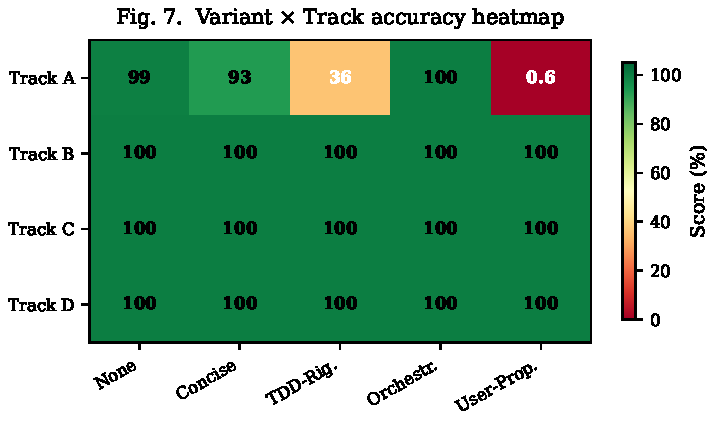
\includegraphics[width=\columnwidth]{figures/fig7_heatmap.pdf}
    \caption{Variant $\times$ Track accuracy heatmap.}
    \label{fig:heatmap}
\end{figure}

\subsection{Provider Dropout Analysis}

The \texttt{user-proposed} variant's Track~A failure (0.56\%) deserves
close examination.
Figure~\ref{fig:dropout} shows the timeline: four of five prompt-response
cycles are terminated by provider-level stream drops before any file edit
is applied.

\begin{figure}[t]
    \centering
    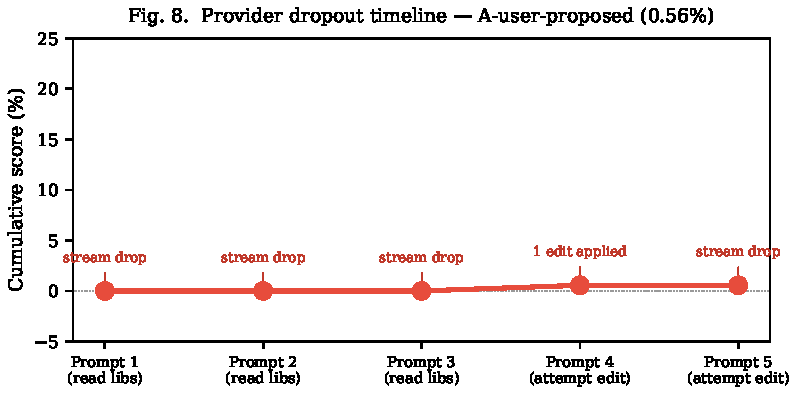
\includegraphics[width=\columnwidth]{figures/fig8_dropout.pdf}
    \caption{Provider dropout timeline for A-user-proposed. Four of five
             cycles terminated by stream drops.}
    \label{fig:dropout}
\end{figure}

This failure is \emph{not} an instruction-quality problem: the tiered
protocol itself is sound, but its front-loaded analysis phase keeps the
agent in long reasoning turns that are vulnerable to stream interruptions.
When the provider is stable (as in Tracks~B/C/D), the variant performs
perfectly.

%% ══════════════════════════════════════════════════════════════════════════════
\section{Discussion}
\label{sec:discussion}

\subsection{Instruction Complexity vs.\ Task Breadth}
Our results reveal a crossover: simple tasks (Tracks~B/C/D, Round~1) are
best served by minimal or no instructions, while breadth-under-deadline
tasks (Track~A) benefit from orchestration-heavy protocols that enable
parallelism.
This suggests that the optimal instruction file is \emph{task-dependent},
not universally optimal.

\subsection{Provider Reliability as Confounding Variable}
The \texttt{user-proposed} variant's Track~A failure demonstrates that
provider reliability can dominate instruction quality.
In production deployments, retry logic and provider failover are at least
as important as prompt design.
We recommend that future benchmarks report provider availability and
stream-drop rates alongside accuracy metrics.

\subsection{Speed--Accuracy Pareto Frontier}
The \texttt{orchestrator-heavy} variant and the control (\texttt{none})
define the Pareto frontier: the former for maximum accuracy, the latter
for maximum speed on narrow tasks.
The \texttt{tdd-rigorous} variant, despite its theoretical appeal, falls
below the frontier on breadth tasks due to excessive diagnostic overhead.

\subsection{Lessons for Practitioners}
\begin{enumerate}
    \item For \textbf{narrow, single-file tasks}: use minimal instructions
          (or none). The control scored 99.86\% overall.
    \item For \textbf{broad, multi-library tasks}: use orchestration-heavy
          instructions that encourage parallel subagent use.
    \item For \textbf{time-critical deployments}: avoid front-loaded
          analysis protocols; they are vulnerable to provider drops.
    \item Always implement \textbf{retry logic}: provider stream drops are
          common and confound instruction quality.
\end{enumerate}

%% ══════════════════════════════════════════════════════════════════════════════
\section{Released Artifacts}
\label{sec:artifacts}

As a practical outcome of this benchmark, we release three reusable OpenCode
specialist agents:

\begin{itemize}
    \item \texttt{arena-runner}: launches and scores benchmark runs with
          provider-dropout retry logic and results-only commits.
    \item \texttt{arena-analyst}: evidence-first leaderboard aggregation
          with cap/DNF honesty markers.
    \item \texttt{suite-author}: authors new task suites under the
          repository's verified integrity conventions.
\end{itemize}

These agents are installed globally via a single PowerShell script and
include slash commands (\texttt{/run-arena}, \texttt{/analyze-arena}) for
interactive use.
They are deliberately shipped without a pinned model, as provider model
IDs were observed to rotate during the experiment
(\texttt{opencode-go/ox-alpha-free} vanished mid-session).

%% ══════════════════════════════════════════════════════════════════════════════
\section{Conclusion}
\label{sec:conclusion}

This paper presented the first empirical comparison of \texttt{AGENTS.md}
instruction-file variants for LLM-based coding agents.
Across 25 tasks, 4 thematic tracks, and 5 instruction variants, we found:

\begin{enumerate}
    \item On narrow tasks, instruction complexity adds overhead without
          improving accuracy; no instructions is competitive.
    \item On breadth-under-deadline tasks, orchestration-heavy instructions
          that enable parallelism are the only variant to achieve perfect
          accuracy.
    \item Provider reliability is a confounding variable that can dominate
          instruction quality for protocols with long reasoning turns.
    \item The speed--accuracy trade-off is real and measurable: the fastest
          variant (5.9~min on Round~1) is 40\% slower than the slowest on
          Round~2 Track~A, but 64\% faster on Track~C.
\end{enumerate}

Future work should explore adaptive instruction files that adjust complexity
based on task difficulty, and should include provider-failover mechanisms as
a first-class experimental variable.

%% ══════════════════════════════════════════════════════════════════════════════
\section*{Acknowledgment}

The author thanks the OpenCode development team for the open-source agent
framework, and the providers behind the \texttt{ox-alpha-free} model for
research access.

\bibliographystyle{IEEEtran}
\begin{thebibliography}{10}

\bibitem{cursor}
Cursor AI, ``Cursor: The AI-first code editor,'' 2024.
\url{https://cursor.sh}

\bibitem{aider}
P.~Gauthier, ``Aider: AI pair programming in your terminal,'' 2024.
\url{https://aider.chat}

\bibitem{opencode}
OpenCode, ``OpenCode: AI coding agent,'' 2025.
\url{https://opencode.ai}

\bibitem{swebench}
C.~E.~Jimenez \textit{et~al.}, ``SWE-bench: Can language models resolve
real-world GitHub issues?'' in \textit{Proc. ICLR}, 2024.

\bibitem{humaneval}
M.~Chen \textit{et~al.}, ``Evaluating large language models trained on
code,'' \textit{arXiv:2107.03374}, 2021.

\bibitem{mbpp}
J.~Austin \textit{et~al.}, ``Program synthesis with large language
models,'' \textit{arXiv:2108.07732}, 2021.

\bibitem{codellama}
B.~Rozi\`ere \textit{et~al.}, ``Code Llama: Open foundation models for
code,'' \textit{arXiv:2308.12950}, 2023.

\bibitem{copilot}
GitHub, ``GitHub Copilot: Your AI pair programmer,'' 2023.
\url{https://github.com/features/copilot}

\bibitem{instructgpt}
L.~Ouyang \textit{et~al.}, ``Training language models to follow instructions
with human feedback,'' in \textit{Proc. NeurIPS}, 2022.

\bibitem{systemprompt}
J.~Wei \textit{et~al.}, ``Chain-of-thought prompting elicits reasoning in
large language models,'' in \textit{Proc. NeurIPS}, 2022.

\end{thebibliography}

\end{document}
